%!TeX program = xelatex
\documentclass[12pt,hyperref,a4paper,UTF8]{ctexart}
\usepackage{compiler_versions_recognition}
\usepackage{inputenc}
\usepackage[british,UKenglish]{babel}
\usepackage{amsmath}
\usepackage{algorithm}%算法
\usepackage{algorithmic}%算法
\usepackage{subfiles}%分文件编写章节
\usepackage{booktabs}
\usepackage{titlesec}
\usepackage{color}
\usepackage{graphicx}
\usepackage{subfigure}%子图
\usepackage{subcaption}%子图
\usepackage{fancyref}
\usepackage{hyperref}%超链接
\usepackage{float}%浮动图片
\usepackage{scrextend}
\usepackage{setspace}
\usepackage{xargs}
\usepackage{multicol}
\usepackage{nameref}
\usepackage{longtable}
\usepackage{sectsty}
\usepackage{booktabs}
\usepackage{longtable}
\usepackage{multicol}
\usepackage{multirow}
\usepackage{appendix}
\usepackage{listings}

\newcommand\tab[1][1cm]{\hspace*{#1}}
\hypersetup{colorlinks=true, linkcolor=blue}
\interfootnotelinepenalty=10000
% -------------------------允许算法跨页-------------
\makeatletter
\newenvironment{breakablealgorithm}
  {% \begin{breakablealgorithm}
   \begin{center}
     \refstepcounter{algorithm}% New algorithm
     \hrule height.8pt depth0pt \kern2pt% \@fs@pre for \@fs@ruled
     \renewcommand{\caption}[2][\relax]{% Make a new \caption
       {\raggedright\textbf{\ALG@name~\thealgorithm} ##2\par}%
       \ifx\relax##1\relax % #1 is \relax
         \addcontentsline{loa}{algorithm}{\protect\numberline{\thealgorithm}##2}%
       \else % #1 is not \relax
         \addcontentsline{loa}{algorithm}{\protect\numberline{\thealgorithm}##1}%
       \fi
       \kern2pt\hrule\kern2pt
     }
  }{% \end{breakablealgorithm}
     \kern2pt\hrule\relax% \@fs@post for \@fs@ruled
   \end{center}
  }
\makeatother


\newcommand{\cleancode}[1]{\begin{addmargin}[3em]{3em}\texttt{\textcolor{cleanOrange}{#1}}\end{addmargin}}
\newcommand{\cleanstyle}[1]{\text{\textcolor{cleanOrange}{\texttt{#1}}}}


\usepackage[colorinlistoftodos,prependcaption,textsize=footnotesize]{todonotes}
\newcommandx{\commred}[2][1=]{\textcolor{Red}
{\todo[linecolor=red,backgroundcolor=red!25,bordercolor=red,#1]{#2}}}
\newcommandx{\commblue}[2][1=]{\textcolor{Blue}
{\todo[linecolor=blue,backgroundcolor=blue!25,bordercolor=blue,#1]{#2}}}
\newcommandx{\commgreen}[2][1=]{\textcolor{OliveGreen}{\todo[linecolor=OliveGreen,backgroundcolor=OliveGreen!25,bordercolor=OliveGreen,#1]{#2}}}
\newcommandx{\commpurp}[2][1=]{\textcolor{Plum}{\todo[linecolor=Plum,backgroundcolor=Plum!25,bordercolor=Plum,#1]{#2}}}

\def\code#1{{\tt #1}}

\def\note#1{\noindent{\bf [Note: #1]}}

\makeatletter
%% The "\@seccntformat" command is an auxiliary command
%% (see pp. 26f. of 'The LaTeX Companion,' 2nd. ed.)
\def\@seccntformat#1{\@ifundefined{#1@cntformat}%
   {\csname the#1\endcsname\quad}  % default
   {\csname #1@cntformat\endcsname}% enable individual control
}
\let\oldappendix\appendix %% save current definition of \appendix
\renewcommand\appendix{%
    \oldappendix
    \newcommand{\section@cntformat}{\appendixname~\thesection\quad}
}
\makeatother


%%-------------------------------正文开始---------------------------%%
\begin{document}
%%-----------------------封面--------------------%%
\cover
%%------------------摘要-------------%%
%\begin{abstract}
%
%在此填写摘要内容
%
%\end{abstract}

\thispagestyle{empty} % 首页不显示页码

%%--------------------------目录页------------------------%%
\newpage
\tableofcontents

%%------------------------正文页从这里开始-------------------%
\newpage
\section{问题提出}
\subsection{相关背景介绍}
电子计算机自诞生以来,经历了快速而显著的发展。在短短的百年时间里,计算机在体积、能耗、计算速度和应用能力等方面都发生了巨大变化。
然而,要充分发挥计算机的潜力,必须使用能够被其解释和执行的指令序列,即程序。
最初,这些程序是通过机器语言编写的,但由于其不直观,极大地限制了计算机的普及。为了解决这一问题,1957年,第一个自动编译器FORTRAN诞生了。
此后,许多性能更高且支持接近自然语言的编译器相继被设计出来,如C/C++编译器GCC,Clang。编译器的出现极大地推动了计算机在现代社会的广泛应用。

\par
为了便于使用计算机,人们首先需要按照特定规则(即程序设计语言,例如C++语言)将待执行的指令以特定顺序编写成源代码。这些源代码随后通过编译器自动翻译(即编译)为一系列机器语言指令(即汇编语言),最后通过链接器各种库文件(链接库),生成可执行程序,并提交给计算机执行。
源代码是程序的初始形式,通常以高级编程语言编写,具有良好的可维护性,并且形式上更加接近自然语言。而汇编语言则是一种机器语言,本质上是由01一一序列映射成的低级程序设计语言,如\autoref{fig:ass}所示,一条汇编语言语句通常由操作码,操作数组成,操作题提供本条指令要执行的操作,而操作数提供数据的来源,\autoref{fig:ass}中展示的汇编语句的作用是 将寄存器rdx和rax中的数据取出来相加,然后把结果放回到rdx寄存器中。
\begin{figure}[H]
    \centering
    
\includegraphics[width=0.8\textwidth]{figures/ass.png}
    \caption{汇编语句的组成}
    \label{fig:ass}
\end{figure}
编译器则是将源代码翻译为机器语言的工具,汇编语言作为机器语言的中间形式,提供了一种更易于理解和操作的方式。编译器的工作流程如\autoref{fig:compiler}所示。编译器会根据源代码构建一个语法树,然后根据语法树的规则转翻译源代码为汇编语言代码。不同版本的编译器在转译时有部分不同的处理方式,例如通过指令调度算法来减少跳转,寄存器换名技术来消除数据冲突。
\begin{figure}
    \centering
    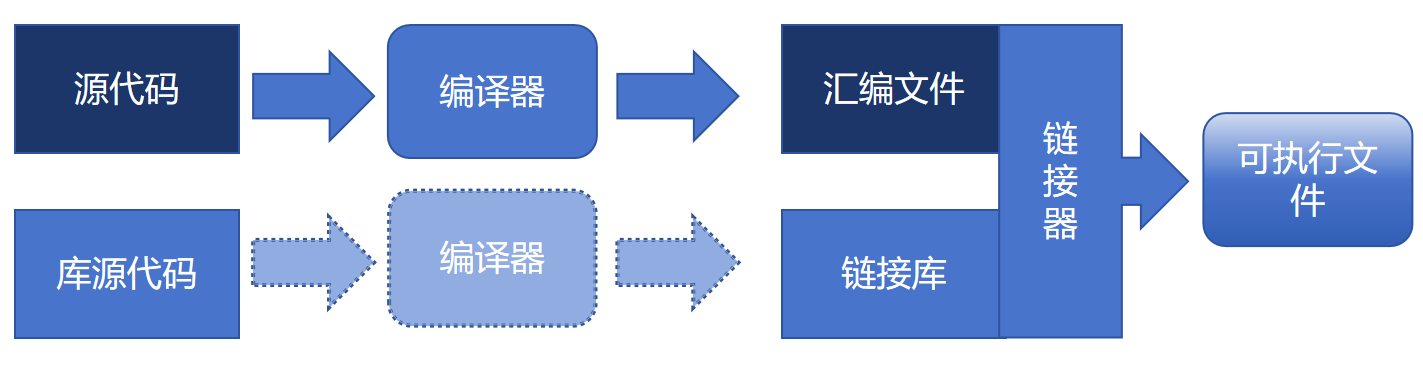
\includegraphics[width=0.8\textwidth]{figures/compiler.png}
    \caption{编译器的工作流程}
    \label{fig:compiler}
\end{figure}
随着编程语言的演变,编译器也在不断更新。例如,GCC(GNU Compiler Collection)已经更新到13.2.0版本。不同版本的编译器在编译同一程序时可能产生不同的编译结果;即使是相同版本的编译器,使用不同的编译选项也会导致编译结果的差异。因此,研究如何利用这些差异来区分编译器的版本具有重要意义。
\par
\subsection{问题重述}
\textbf{问题1}:使用多种不同版本的GCC C++编译器默认编译选项,编译附件中的程序源代码1。任务核心是对比这些不同版本编译器的输出结果,识别并记录体现编译器版本差异的特征。

\textbf{问题2}:将识别出的编译器版本特征转化为实际可用的判别函数。

\textbf{问题3}:使用不同版本的GCC C++编译器编译附件中的程序源代码2,应用已开发的判别函数测试其效果,验证其在不同源代码上的普适性和准确性,并研究更加广泛有效的判别函数。

\textbf{问题4}:提出几条建议以提高判别函数的性能,包括提升判别函数的区分度和增强对不同源代码的泛化能力。

\vspace*{1cm}

\section{问题3}
\subsection{决策树模型分析}
决策树模型作为一种简单且直观的机器学习算法,广泛应用于分类和回归任务。然而,尽管其易于理解和解释,决策树模型也存在一些固有的缺陷,决策树模型存在以下几个缺陷:
\begin{itemize}
	\item 容易过拟合:决策树模型在处理复杂数据集时,容易出现过拟合问题。这是因为决策树模型在构建过程中会根据数据的分布来选择分裂点,如果数据集过于复杂,决策树可能会生成\textbf{过深的树结构},从而导致模型过拟合,泛化能力较差。

	      \tbox{\autoref{fig:fit_status}展示了不同拟合状态的大致情况,过拟合是模型完全拟合了训练数据,把训练的数据的噪声也当做数据的统计特征,从而导致在训练集的误差很低,但是在测试集的误差很高。}
	\item 对数据噪声敏感:决策树对数据中的噪声和异常值非常敏感。这是因为决策树在构建过程中会根据数据的分布来选择分裂点,噪声和异常值可能导致树的结构发生较大变化,从而影响模型的稳定性和准确性。
	\item 不稳定:由于决策树的构建过程是基于局部最优的贪心算法,因此对数据的变化非常敏感,小的输入数据变化可能导致决策树结构的显著变化。
	\item 计算复杂度:在特征数量较多或数据集较大时,决策树的构建过程可能会非常耗时。这是因为每次分裂都需要计算所有可能分裂点的增益,从而选择最佳分裂点。
\end{itemize}
\begin{figure}[H]
	\centering
	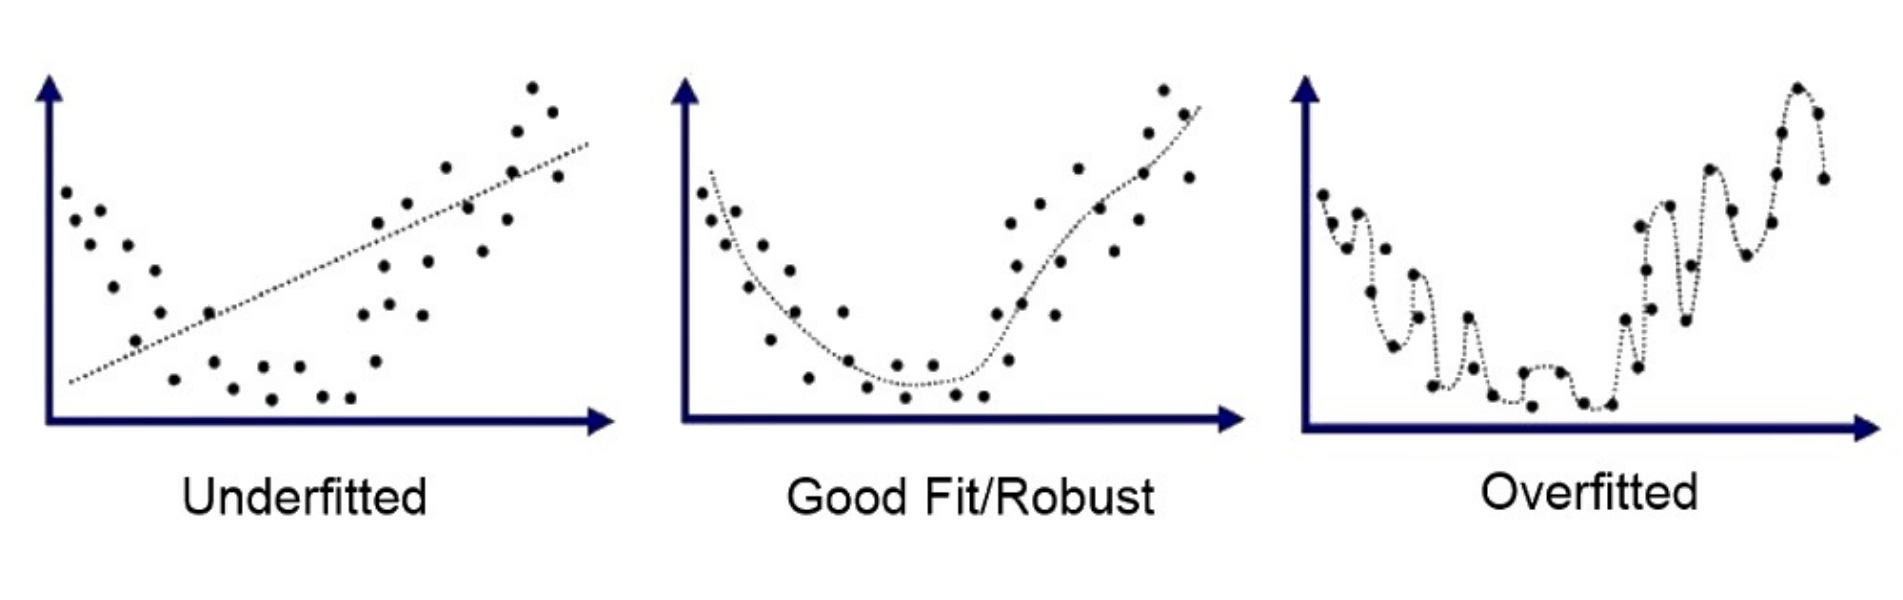
\includegraphics[width=0.8\textwidth]{figures/fit_status.png}
	\caption{不同拟合状态}
	\label{fig:fit_status}
\end{figure}

并且,在我们的实验中,我们发现如果只使用附件1或者是附件2来构建模型,模型的预测结果将会趋向于随机猜测,而非根据编译器的特征进行预测。
\par
从数据的分布来看,我们使用t-SNE算法对数据进行降维可视化,t-分布邻域嵌入(t-distributed Stochastic Neighbor Embedding,t-SNE)\cite{JMLR:v9:vandermaaten08a}是一种非线性降维技术,特别适用于高维数据的可视化。t-SNE通过将高维数据映射到低维空间,同时\textbf{尽可能保持数据点之间的局部结构},从而揭示数据的内在结构和模式。t-ESN算法通过优化KL散读来最小化高维空间和低维空间之间的分布差异,从而实现降维。t-SNE的优化目标是最小化高维空间和低维空间之间的KL散度,KL散度定义如下:
\begin{equation}
	C=KL(P||Q)=\sum_i\sum_jp_{ij}\log\frac{p_{ij}}{q_{ij}},
\end{equation}
其中,$p_{ij}$是高维数据点$x_i$和$x_j$之间的相似度,在高纬空间中,t-SNE算法使用高斯分布来衡量高维空间中点对之间的相似性。$q_{ij}$是低维数据点$y_i$和$y_j$之间的相似度。在低维空间中,t-SNE使用学生t分布(t-distribution)来计算点对之间的相似性。这个分布的长尾特性使得它能够更好地捕捉低维空间中的局部结构。t-SNE通过梯度下降算法优化该目标,C对于低维数据的梯度为
\begin{equation}
	\frac{\delta C}{\delta y_i}=4\sum_j(p_{ij}-q_{ij})(y_i-y_j)\left(1+\|y_i-y_j\|^2\right)^{-1},
\end{equation}
最后使用梯度更新低维数据点$y_i$
\begin{equation}
	y_i^{(t+1)}=y_i^{(t)}+\eta\frac{\delta C}{\delta y_i},
\end{equation}
其中$\eta$是学习率。在t-SNE算法中,还引入了\textbf{动量}来进一步优化低位数据点的表示:
\begin{equation}
	momentum=\alpha(y_i^{(t)}-y_i^{(t-1)}).
\end{equation}
动量项通过在更新过程中加入前几次更新的累积效果,可以帮助算法在梯度方向上更快地移动,并且通过平滑更新路径,能够有效减少震荡,使得优化过程更加稳定。加入动量后的更新公式为
\begin{equation}
	y_i^{(t+1)}=y_i^{(t)}+\eta\frac{\delta C}{\delta y_i}+\alpha(y_i^{(t)}-y_i^{(t-1)})m
\end{equation}
综上所述,T-SNE算法流程如\autoref{alg:tsne}所示。
\begin{algorithm}[H]
	\caption{t-SNE}
	\label{alg:tsne}
	\begin{algorithmic}
		\REQUIRE 数据集$X$,目标维度$k$,,优化参数:迭代次数$T$,学习率$\eta$,动量参数$\alpha$
		\ENSURE  低维数据$\mathcal{Y}$

		\STATE 计算高维数据之间的相似度$p_{j|
					i}$
		\[
		p_{j|i}=\frac{\exp\left(-\|x_i-x_j\|^2/2\sigma_i^2\right)}{\sum_{k\neq i}\exp\left(-\|x_i-x_k\|^2/2\sigma_i^2\right)}
		\]
		其中$\sigma_i$是以$\boldsymbol{x_i}$为中心的高斯分布的方差,通过二分搜索确定
		\STATE 从$\mathcal{N}(0,10^{-4}I)$从采样$\mathcal{Y}^{(0)}={y_1,y_2,\cdots,y_n}$
		\FOR {$i=1$ to $T$}
		\STATE 计算低维数据之间的相似度$q_{j|i}$
		\[q_{j|i}=\frac{(1+\|y_i-y_j\|^2)^{-1}}{\sum_{k\neq i}(1+\|y_i-y_k\|^2)^{-1}}\]
		\STATE 计算梯度
		\[
			\frac{\delta C}{\delta y_i}=4\sum_j(p_{ij}-q_{ij})(y_i-y_j)\left(1+\|y_i-y_j\|^2\right)^{-1}.
		\]
		\STATE 更新$y_i$
		\[
			y_i^{(t+1)}=y_i^{(t)}+\eta\frac{\delta C}{\delta y_i}+\alpha(y_i^{(t)}-y_i^{(t-1)})
		\]
		\ENDFOR
	\end{algorithmic}
\end{algorithm}
我们使用Scikit-learn\cite{scikit-learn}实现t-SNE算法的可视化,结果如\autoref{fig:tsne}所示。
\begin{figure}[H]
	\centering
	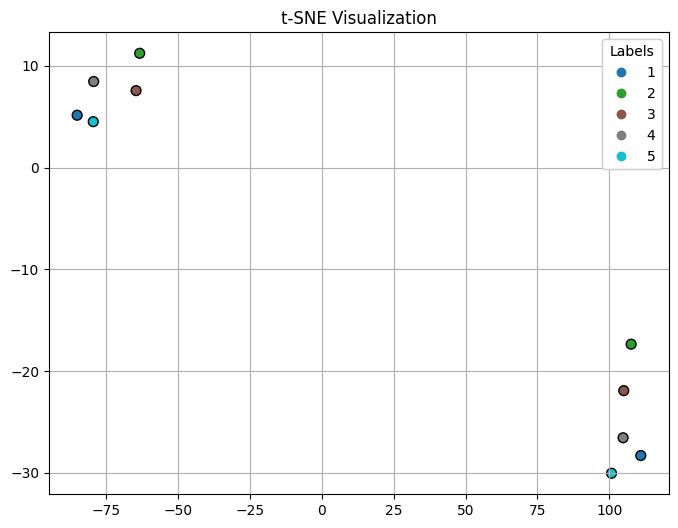
\includegraphics[width=0.7\textwidth]{figures/tsne.png}
	\caption{t-SNE降维可视化}
	\label{fig:tsne}
\end{figure}
可以发现,附件1和附件2在整体上的数据分布相差很远,并且在局部上同一个源文件的不同版本之间也没有明显的分布规律。这也是导致决策树模型无法准确预测的原因之一。
\vspace{1cm}
\subsection{模型改进}
通过对决策树模型和数据分布的分析,我们发现以下问题
\begin{itemize}
	\item \textbf{训练数据不具备广泛性}:原有的训练数据少,并且类型单一,无法体现编译器在编译技术上的优化方法和特点
	\item \textbf{模型本身的缺陷}:单纯的决策树模型容易过拟合:在没有剪枝方法的情况下,决策树的深度容易过深,导致模型过拟合,泛化能力较差。但是如果使用剪枝方法,则决策树又容易欠拟合,导致模型的准确率较低
\end{itemize}
\par
针对训练的问题,我们需要根据不同版本编译器的特点来对应生成数据。使用对应生成的数据训练模型,可以使得模型能够捕捉到不同版本编译器在编译技术和优化方法上的差异。我们注意到一个软件:\textbf{CSmith}。该软件是用于编译器压力测试的随机程序生成器。它专门用于生成程序源代码,以帮助测试和验证编译器的正确性和稳健性。生成的代码有以下特点:
\begin{itemize}
	\item 1.CSmith生成的代码涵盖了编程语言的大部分特性,包括指针、数组、结构体以及复杂的控制流结构等。这种广泛的覆盖性有助于发现不同版本编译器在编译技术上的差异。
	\item 2.随机性和多样性:生成的代码是随机的,这意味着每次运行CSmith都会产生不同的程序。这进一步提高生成的代码的随机性和多样性。
\end{itemize}
基于CSmith,我们生成了1000个随机程序,并使用不同版本的编译器对这些程序进行编译,得到了1000个数据样本。
\par
由于我们引入了大量数据,并且决策树模型存在固有的缺陷,因此我们考虑使用\textbf{集成模型}来构建判别函数。集成模型是一种强大的机器学习方法,首先构建多个弱分类器,然后在把这些弱分类器的分类结果进行加权,得到一个强分类器。\autoref{fig:ensemble}显示了集成模型的基本原理。
\begin{figure}
	\centering
	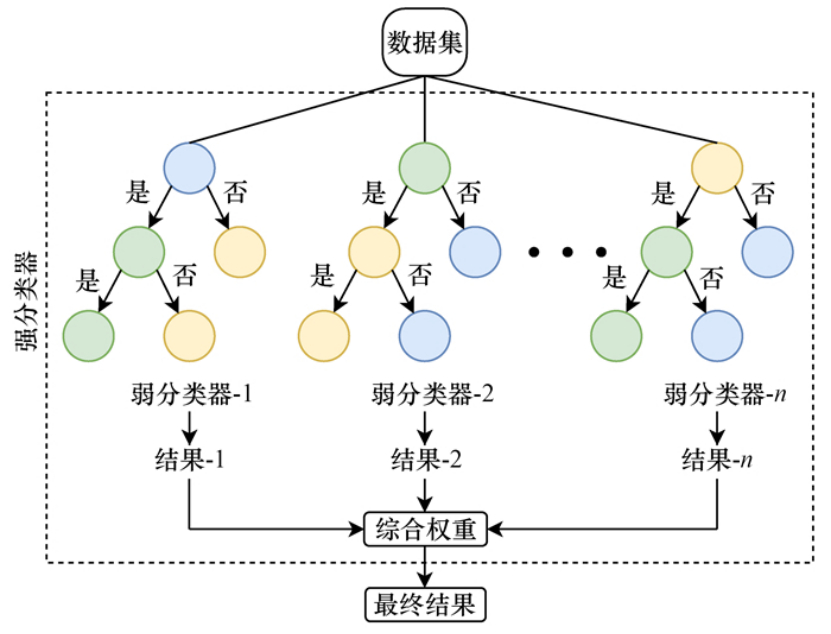
\includegraphics[width=0.7\textwidth]{figures/ensemble.png}
	\caption{集成模型的基本原理}
	\label{fig:ensemble}
\end{figure}
在选择机器学习模型时,我们主要考虑以下几个关键特性:\textbf{训练速度快、能够处理高维数据以及具备良好的泛化能力}。基于这些特性,我们选择了\textbf{XGBoost}模型。\textbf{XGBoost(Extreme Gradient Boosting)}\cite{10.1145/2939672.2939785}是一种高效且灵活的梯度提升框架,通过集成决策树模型并逐步优化,展现出卓越的性能和可扩展性,尤其在处理大规模数据集时表现优异。XGBoost的主要优点包括:
\begin{itemize}
	\item 高性能:XGBoost通过直方图优化、GPU加速以及数据/特征并行等技术,大幅提升了训练效率,相较于一般的集成模型,它能够更快速地完成训练过程。
	\item 灵活性:作为一个集成决策树模型,XGBoost不仅能够自动处理缺失值,还能处理数值型和类别型等多种类型的数据。这种灵活性使其非常契合我们数据集的特点。
	\item 准确性:XGBoost通过拟合决策树的预测残差,逐步优化树模型的结构和权重,从而提升预测准确性。这种逐步优化的方式有效地提高了模型的整体性能。
	\item 可解释性:XGBoost提供了特征重要性评估和模型解释功能,使我们能够更直观地理解模型的预测结果,以及各特征对预测结果的影响。这种可解释性对于模型的应用和改进具有重要意义。
\end{itemize}
通过这些优势,XGBoost成为我们在处理复杂数据集和追求高效、准确预测时的理想选择。
XGBoost的原理如下:
假设已经训练了$t-1$个模型,现在准备增加一个模型$f_t(x)$,使得目标函数:
\begin{equation}
	\mathcal{L}(F_{t-1}+\alpha f_t)=\sum_{i=1}^{n}l(y_i,\hat{y}^{(t)})+\Omega(f_t),
\end{equation}
最小化,其中$\hat{y}^{(t)}=F_{t-1}(x)+f_t(x)$,$\Omega(f_t)$是正则化项,$l(y_i,\hat{y}^{(t)})$是损失函数,$n$ 是样本数量。我们对损失函数$l(y_i,\hat{y}^{(t)})$在$F_{t-1}(x)+f_t(x)$处进行二阶泰勒展开,并且忽略余项,那么我们可以得到
\begin{equation}
	l(y_i,\hat{y}^{(t)})\approx\sum_{i=1}^{n}\left[l\left(y_{i},\hat{y}_{i}^{(t-1)}\right)+g_{i}f_{t}(x_{i})+\frac{1}{2}h_{i}f_{t}^{2}(x_{i})\right],
\end{equation}
其中$g_i=\nabla_{\hat{y}^{(t-1)}}l\left(y_i,\hat{y}_i^{(t-1)}\right)\quad h_i=\nabla_{\hat{y}^{(t-1)}}^2l\left(y_i,\hat{y}_i^{(t-1)}\right)$,对于每个叶子结点的预测
\begin{equation}
	f_t(x)=w_{q(x)},w\in\mathbb{R}^T,q\colon\mathbb{R}^d\mapsto\{1,2,...,T\},,,,,
\end{equation}
其中$T$是叶子结点的个数,$q(x)$是样本$x$在树中的叶子结点的索引(因为每个样本最终都会落到某个叶子节点上),$w$是叶子结点的权重,那么我们就可以定义正则化函数:
\begin{equation}
	\Omega(f_t)=\gamma T+\frac{1}{2}\lambda\sum_{i=1}^{T}w_i^2,
\end{equation}
$\gamma$和$\lambda$是超参数,分别控制叶子结点的个数和叶子结点的惩罚权重,最终的优化目标为
\begin{equation}
	\begin{aligned}
		\mathcal{L}^{(t)} & \simeq\sum_{i=1}^{n}\left[l\left(y_{i},\hat{y}_{i}^{(t-1)}\right)+g_{i}f_{t}(x_{i})+\frac{1}{2}h_{i}f_{t}^{2}(x_{i})\right]+\Omega(f_{t})
		\\
		                  & =\sum_{i=1}^{n}\left[g_{i}f_{t}(x_{i})+\frac{1}{2}h_{i}f_{t}^{2}(x_{i})\right]+\gamma T+\frac{1}{2}\lambda\sum_{j=1}^{T}w_{j}^{2}+co
		\\
		                  & =\sum_{j=1}^{T}\left[(\sum_{i\in I_{i}}g_{i})w_{j}+\frac{1}{2}(\sum_{i\in I_{i}}h_{i}+\lambda)w_{j}^{2}\right]+\gamma T+const
	\end{aligned}
\end{equation}
其中$I_j$是样本集合$\{i|q(x_i)=j\}$,也就是由于每个样本最终都会落到某个叶子结点上,因此把对样本的求和转换为对叶子结点的求和,并且$l(y_i,y^{(t-1)})$是已经确定的常数,因此最终优化目标是
\begin{equation}
	\mathcal{L}^{(t)}=\sum_{j=1}^{T}\left[(\sum_{i\in I_{i}}g_{i})w_{j}+\frac{1}{2}(\sum_{i\in I_{i}}h_{i}+\lambda)w_{j}^{2}\right]+\gamma T
\end{equation}
这是一个关于$w_i$的二次函数,可以通过求导得到最优解,令
\begin{equation}
	G_j=\sum_{i \in I_j}g_i\quad H_j=\sum_{i \in I_j}h_i,
\end{equation}
则优化目标的闭式解为
\begin{equation}
	w_{j}^{*}=-\frac{G_{j}}{H_{j}+\lambda}\quad \mathcal{L}^{(t)}=-\frac{1}{2}\sum_{i=1}^{T}\:\frac{G_{j}^{2}}{H_{j}+\lambda}+\gamma T,
\end{equation}
那么在构建决策树时,我们可以通过贪心算法,从根节点开始,对每个叶子结点,计算其最优的权重$w_j$,然后计算损失函数,
\begin{equation}
	\text{Gain}=\frac{1}{2}(\frac{G_{L}^{2}}{H_{L}+\lambda}+\frac{G_{R}^{2}}{H_{R}+\lambda}-\frac{(G_{L}+G_{R})^{2}}{H_{L}+H_{R}+\lambda})-\gamma,
\end{equation}
其中$G_L,H_L$和$G_R,H_R$分别是左右子树的梯度值,最后选择最优的划分特征和划分点,递归构建树,直到满足停止条件。
在本题中,由于是分类问题,我们使用交叉熵作为损失函数,
\begin{equation}
	l(y_i,\hat{y}_i^{(t-1)})=-\left(y_i\log(\hat{y}_i^{(t-1)})+(1-y_i)\log(1-\hat{y}_i^{(t-1)})\right)
\end{equation}
则该损失函数的梯度和二阶导数分别为
\begin{equation}
	g_i=\hat{y}_i^{(t-1)}-y_i ,\quad h_i=\hat{y}_i^{(t-1)}(1-\hat{y}_i^{(t-1)}),
\end{equation}

最终,XGBoost的算法如\autoref{alg:xgboost}所示。
\begin{algorithm}[H]
	\caption{XGBoost}
	\label{alg:xgboost}
	\begin{algorithmic}[1]
		\REQUIRE 超参数:$\lambda$ 和 $\gamma$。特征$X$,标签$Y$。停止条件:树的最大深度$K$。
		\ENSURE 集成模型XGBoost

		\STATE \textbf{计算梯度和二阶导数}:
		\FOR{每个样本 $i$}
		\STATE 计算损失函数的一阶梯度 $g_i$ 和二阶导数 $h_i$。
		\ENDFOR
		\STATE \textbf{遍历所有特征}:
		\FOR{每个特征 $j$}
		\STATE 计算所有可能的分裂点。
		\FOR{每个分裂点}
		\STATE 将数据集分为左子集 $L$ 和右子集 $R$。
		\STATE 计算左子集和右子集的梯度和二阶导数之和:
		\STATE $G_L = \sum_{i \in L} g_i, \quad H_L = \sum_{i \in L} h_i$
		\STATE $G_R = \sum_{i \in R} g_i, \quad H_R = \sum_{i \in R} h_i$
		\STATE 计算分裂增益:
		\STATE $\text{Gain} = \frac{1}{2}\left(\frac{G_L^2}{H_L + \lambda} + \frac{G_R^2}{H_R + \lambda} - \frac{(G_L + G_R)^2}{H_L + H_R + \lambda}\right) - \gamma$
		\ENDFOR
		\ENDFOR
		\STATE \textbf{选择最佳分裂点}:
		\STATE 对于每个特征,选择具有最大增益的分裂点。
		\STATE 在所有特征中,选择增益最大的分裂点作为最终的分裂点。
		\STATE \textbf{递归分裂}:
		\STATE 对于新的左子树和右子树,重复步骤2至5,直到满足停止条件
	\end{algorithmic}
\end{algorithm}
\par
对于$d$个特征,每个特征,都可以以$O(1)$的速度构建计算增益,每一层都需要$n\log n$的时间排序选出最佳特征,一共$K$层,因此整个XGBoost算法的时间复杂度为$O(Kdn\log{n})$

\vspace*{1cm}
\section{问题四}
提高由编译结果区分编译器版本的判别函数性能的建议:
\vspace*{1cm}
\subsection{自动特征提取}
特征工程将原始数据转化为更适合模型学习的特征的过程,直接影响模型的性能和准确性。然而,传统的手动特征工程存在一些缺陷。首先,手动特征工程依赖于领域专家的知识和经验,这将导致特征选择的主观性和局限性。其次,手动提取特征通常是一个耗时且繁琐的过程,尤其在高维数据或复杂数据结构的情况下,难以保证全面和高效。因此,如果要提高模型的区分度和性能,我们可以考虑采用深度学习技术来进行自动特征提取我们构想了一个基于协同注意力机制的模型。具体来说,首先将源文件和对应的汇编文件转换为词向量嵌入表示。然后,利用基于 Transformer 的自注意力机制来捕捉文件内部的语义特征。为了更好地理解源文件与汇编文件之间的关系,进一步采用 Cross-Attention 机制来提取它们之间的语义相似性和结构相异性。这种方法的优势在于,它能够自动捕捉不同编译器版本之间在语义和结构上的细微差异,这些差异可以作为有效的特征,用于构建高效的分类模型。
\vspace{1cm}
\subsection{增加数据集多样性}
考虑到不同领域的源代码会存在很大的差异,例如同为C++程序代码,后端服务器代码往往倾向于网络和IO操作,而游戏的代码则会包含到大量的图形渲染和物理计算,因此不同领域的源代码在同一个版本的编译器编译的编译结果存在很大差异。此外,即使是同一个领域的源代码,不同规模的源代码之间也会存在非编译器造成的差异。最后编译器版本之间的差距主要是体现在对于不同版本的语言支持以及静态代码优化技术,而后者一般要通过编译指令开启代码优化才能体现。鉴于以上分析,我们可以通过以下几种方式来增加数据集的多样性,提高模型的泛化能力:
\begin{itemize}
    \item 不同类型的程序:收集多种类型的程序(如计算密集型、IO 密集型、混合型)进
    行编译,提取汇编结果。
    \item 不同规模的程序:从小规模到大规模的程序进行编译,确保模型能泛化到不同复
    杂度的代码。
    \item 编译优化级别:使用不同的优化级别(如-O0,-O1,-O2,-O3)进行编译,捕捉
    编译器在不同优化下的行为差异。
\end{itemize}
\vspace*{1cm}
\subsection{结合静态和动态特征}
除了源代码和汇编代码之外,我们还可以考虑结合静态特征和动态特征来提高模型的区分度。具体来说,我们可以提取以下两类特征:
\begin{itemize}
    \item 静态特征:提取静态汇编特征,如指令频率、寄存器使用率、基本块大小。
    \item 动态特征:运行程序,收集运行时的行为特征,如执行路径、内存访问模式、CPU
    使用率。
 我们可以通过结合静态和动态的特征进行分析,更全面地了解编译器版本之间的差异,提高模型的泛化能力。
\end{itemize}

%%----------- 参考文献 -------------------%%
%在reference.bib文件中填写参考文献,此处自动生成
\newpage
\reference


\end{document}